% ======================================================================
\section{Variable definitions and sources}\label{app:data}

\Cref{tab:vardefs} gives the exact definition, unit and source of each variable used in the analysis.

\begin{table}[htbp]
\centering
\footnotesize
\setlength{\tabcolsep}{3pt}
\caption{Variable definitions and sources.}
\label{tab:vardefs}
\begin{tabular}{>{\raggedright\arraybackslash}p{0.19\linewidth}>{\raggedright\arraybackslash}p{0.37\linewidth}>{\raggedright\arraybackslash}p{0.15\linewidth}>{\raggedright\arraybackslash}p{0.22\linewidth}}
\toprule
Variable & Definition & Unit & Source (series) \\
\midrule
Life expectancy & Life expectancy at birth, total & Years & WDI (SP.DYN.LE00.IN), UN WPP \\
Under-5 mortality & Probability of dying before age five & Per 1{,}000 live births & WDI (SH.DYN.MORT), UN IGME \\
Access to electricity & Share of population with access to electricity & \% & WDI (EG.ELC.ACCS.ZS) \\
Employment & 100 minus the unemployment rate, total, modelled ILO estimate & \% of labour force & WDI (SL.UEM.TOTL.ZS), ILO \\
Secondary enrolment$^a$ & Gross enrolment ratio, secondary & \% & WDI (SE.SEC.ENRR), UNESCO UIS \\
Consumption-based \COtwo{} & Fossil and industrial \COtwo{}, adjusted for emissions embodied in trade, per person & t per person per year & Global Carbon Budget 2025 \\
Production-based \COtwo{} & Territorial fossil and industrial \COtwo{} per person & t per person per year & Global Carbon Budget 2025 \\
GHG including land use & \COtwo, CH$_4$ and N$_2$O including land use, per person & t \COtwo-eq.\ (GWP$_{100}$) & \citet{jones2023} \\
GDP per person & Real GDP per person at purchasing power parity & 2011 int.\ \$ & Maddison Project 2023 \\
Population & Total population & Persons & Our World in Data; WDI \\
Continent & Continent of each country, used for descriptive breakdowns & -- & \texttt{country\_converter} \\
\bottomrule
\end{tabular}
\begin{minipage}{0.95\linewidth}\vspace{3pt}\footnotesize\textit{Notes:} $^a$Robustness check only. WDI: World Development Indicators; WPP: World Population Prospects; IGME: Inter-agency Group for Child Mortality Estimation; UIS: Institute for Statistics. Emissions and GDP were obtained through \citet{owid2025co2}.\end{minipage}
\end{table}

% ======================================================================
\section{Country-level results}\label{app:countries}

\Cref{tab:countries} lists, for every country in the sample, its 2011--2022 averages of emissions and the four social indicators, and its configuration in each period. Countries without consumption-based emissions estimates are listed with their production-based emissions and are unclassified.

\begingroup
\footnotesize
\setlength{\tabcolsep}{4pt}
\begin{longtable}{@{}lrrrrrrccc@{}}
\caption{Country values (2011--2022 means) and configurations by period.}\label{tab:countries}\\
\toprule
Country & CO$_2$ cons. & CO$_2$ prod. & Life exp. & U5MR & Elec. & Empl. & 1990--2000 & 2001--2010 & 2011--2022 \\
\midrule
\endfirsthead
\multicolumn{10}{l}{\textit{(continued)}}\\
\toprule
Country & CO$_2$ cons. & CO$_2$ prod. & Life exp. & U5MR & Elec. & Empl. & 1990--2000 & 2001--2010 & 2011--2022 \\
\midrule
\endhead
\bottomrule
\endfoot
\bottomrule
\endlastfoot
Albania & 2.2 & 1.8 & 78.4 & 9.9 & 100 & 86.3 & SW & SO & SO \\
United Arab Emirates & 28.1 & 24.1 & 81.7 & 7.1 & 100 & 97.5 & SO & MO & MO \\
Argentina & 4.3 & 4.2 & 76.0 & 11.5 & 100 & 91.8 & SO & SO & SO \\
Armenia & 2.5 & 2.1 & 74.6 & 13.8 & 100 & 82.6 & SW & SO & SO \\
Australia & 15.8 & 16.5 & 82.6 & 3.9 & 100 & 94.6 & SO & MO & MO \\
Austria & 10.1 & 7.6 & 81.4 & 3.6 & 100 & 94.7 & MO & MO & MO \\
Azerbaijan & 3.7 & 3.6 & 72.0 & 26.3 & 100 & 94.6 & SO & SO & SO \\
Belgium & 18.0 & 8.7 & 81.2 & 4.0 & 100 & 93.0 & SO & SO & SO \\
Benin & 0.7 & 0.4 & 59.4 & 93.6 & 39 & 98.1 & SW & SW & SW \\
Burkina Faso & 0.2 & 0.2 & 59.1 & 96.9 & 17 & 95.7 & SW & SW & SW \\
Bangladesh & 0.7 & 0.5 & 71.0 & 37.1 & 80 & 95.5 & SW & SW & SW \\
Bulgaria & 5.8 & 6.4 & 74.2 & 7.9 & 97 & 92.1 & SO & SO & SO \\
Belarus & 7.1 & 6.5 & 73.0 & 3.8 & 98 & 94.9 & SO & SO & SO \\
Bolivia & 1.9 & 1.8 & 66.3 & 30.5 & 93 & 96.4 & SW & SW & SO \\
Brazil & 2.5 & 2.4 & 74.8 & 15.9 & 100 & 89.8 & SO & SO & SO \\
Botswana & 5.9 & 2.8 & 64.1 & 47.9 & 65 & 80.2 & SO & SO & SO \\
Canada & 15.5 & 15.3 & 81.7 & 5.3 & 100 & 93.0 & SO & SO & SO \\
Switzerland & 16.9 & 4.6 & 83.3 & 4.2 & 100 & 95.3 & MO & MO & MO \\
Chile & 4.9 & 4.5 & 79.7 & 7.6 & 100 & 92.4 & SO & SO & SO \\
China & 6.5 & 7.4 & 77.2 & 10.0 & 100 & 95.4 & SO & MO & MO \\
Cote d'Ivoire & 0.5 & 0.4 & 58.8 & 83.0 & 65 & 96.5 & SW & SW & SW \\
Cameroon & 0.4 & 0.4 & 60.2 & 85.7 & 61 & 96.3 & SW & SW & SW \\
Colombia & 2.2 & 1.9 & 75.7 & 14.9 & 98 & 89.6 & SO & SO & SO \\
Costa Rica & 2.8 & 1.6 & 79.8 & 9.4 & 100 & 89.8 & MO & SO & SO \\
Cyprus & 7.1 & 5.8 & 81.2 & 3.1 & 100 & 89.2 & MO & MO & SO \\
Czechia & 10.5 & 9.9 & 78.5 & 3.1 & 100 & 95.8 & SO & SO & MO \\
Germany & 10.8 & 9.2 & 80.8 & 3.9 & 100 & 95.7 & SO & SO & MO \\
Denmark & 9.6 & 6.2 & 80.9 & 3.9 & 100 & 93.9 & SO & MO & SO \\
Dominican Republic & 3.7 & 2.3 & 73.0 & 34.4 & 99 & 93.4 & SW & SO & SO \\
Ecuador & 2.6 & 2.4 & 75.6 & 15.1 & 99 & 96.1 & SW & MO & MO \\
Egypt, Arab Rep. & 2.5 & 2.3 & 70.1 & 22.3 & 100 & 89.4 & SW & SO & SO \\
Spain & 6.1 & 5.4 & 83.0 & 3.3 & 100 & 81.0 & SO & SO & SO \\
Estonia & 12.7 & 11.9 & 77.5 & 3.0 & 100 & 92.8 & SO & SO & SO \\
Ethiopia & 0.1 & 0.1 & 64.1 & 61.7 & 40 & 97.2 & SW & SW & SW \\
Finland & 11.0 & 8.3 & 81.4 & 2.5 & 100 & 92.1 & SO & SO & SO \\
France & 7.0 & 5.0 & 82.4 & 4.2 & 100 & 90.9 & SO & SO & SO \\
United Kingdom & 8.6 & 6.1 & 81.0 & 4.5 & 100 & 94.5 & SO & MO & MO \\
Georgia & 3.4 & 2.6 & 73.2 & 10.5 & 100 & 84.8 & SW & SO & SO \\
Ghana & 0.8 & 0.5 & 63.5 & 49.8 & 77 & 96.3 & SW & SW & SW \\
Guinea & 0.4 & 0.3 & 58.5 & 110.1 & 38 & 94.9 & SW & SW & SW \\
Greece & 7.4 & 6.7 & 81.1 & 4.1 & 100 & 79.5 & SO & SO & SO \\
Guatemala & 1.0 & 1.0 & 70.7 & 27.1 & 92 & 97.3 & SW & SW & SW \\
Honduras & 0.9 & 1.1 & 71.2 & 19.6 & 90 & 93.4 & SW & SW & SW \\
Croatia & 5.7 & 4.4 & 77.5 & 4.9 & 100 & 88.3 & SO & SO & SO \\
Hungary & 6.4 & 4.8 & 75.5 & 4.8 & 100 & 93.8 & SO & SO & SO \\
Indonesia & 2.2 & 2.2 & 69.4 & 26.2 & 98 & 95.8 & SW & SW & SO \\
India & 1.5 & 1.7 & 69.4 & 40.7 & 90 & 92.8 & SW & SW & SW \\
Ireland & 9.2 & 7.9 & 81.8 & 3.7 & 100 & 91.0 & SO & SO & SO \\
Iran, Islamic Rep. & 6.7 & 8.0 & 75.6 & 14.9 & 100 & 88.9 & SO & SO & SO \\
Israel & 10.7 & 7.6 & 82.3 & 3.8 & 100 & 95.0 & SO & SO & MO \\
Italy & 7.9 & 5.9 & 82.8 & 3.4 & 100 & 89.5 & SO & SO & SO \\
Jamaica & 2.6 & 2.8 & 71.7 & 18.8 & 96 & 92.8 & SO & SO & SO \\
Jordan & 3.6 & 2.5 & 75.3 & 15.9 & 100 & 84.3 & SO & SO & SO \\
Japan & 10.5 & 9.3 & 83.8 & 2.7 & 100 & 96.8 & MO & MO & MO \\
Kazakhstan & 11.3 & 15.2 & 71.7 & 12.2 & 100 & 94.9 & SO & SO & SO \\
Kenya & 0.6 & 0.3 & 62.2 & 46.2 & 55 & 96.2 & SW & SW & SW \\
Kyrgyz Republic & 2.9 & 1.6 & 71.0 & 21.3 & 100 & 95.5 & SO & SO & SO \\
Cambodia & 1.7 & 0.8 & 69.4 & 30.5 & 69 & 99.6 & SW & SW & SO \\
Korea, Rep. & 13.7 & 12.4 & 82.2 & 3.4 & 100 & 96.6 & SO & MO & MO \\
Kuwait & 24.5 & 24.1 & 79.5 & 9.2 & 100 & 97.6 & MO & MO & MO \\
Lao PDR & 1.2 & 1.9 & 66.9 & 50.9 & 89 & 98.0 & SW & SW & SW \\
Sri Lanka & 1.8 & 0.9 & 76.1 & 8.3 & 96 & 95.6 & SW & SW & MO \\
Lithuania & 7.6 & 4.7 & 74.8 & 4.5 & 100 & 90.9 & SO & SO & SO \\
Latvia & 7.0 & 3.7 & 74.3 & 4.9 & 100 & 90.1 & SO & SO & SO \\
Morocco & 1.9 & 1.7 & 73.1 & 22.3 & 98 & 90.5 & SW & SO & SO \\
Madagascar & 0.2 & 0.1 & 63.1 & 66.4 & 26 & 97.8 & SW & SW & SW \\
Mexico & 4.6 & 3.9 & 73.6 & 15.5 & 99 & 95.8 & SO & SO & SO \\
Mongolia & 10.9 & 11.5 & 70.6 & 18.3 & 91 & 94.1 & SO & SO & SO \\
Mozambique & 0.5 & 0.2 & 59.4 & 74.3 & 27 & 95.8 & SW & SW & SW \\
Mauritius & 5.2 & 3.3 & 74.1 & 15.2 & 100 & 92.8 & SO & SO & SO \\
Malawi & 0.1 & 0.1 & 63.0 & 54.1 & 12 & 94.9 & SW & SW & SW \\
Malaysia & 7.8 & 7.7 & 75.4 & 8.1 & 100 & 96.5 & SO & MO & MO \\
Namibia & 4.0 & 1.4 & 60.8 & 50.4 & 51 & 79.9 & SW & SW & SO \\
Nigeria & 0.7 & 0.6 & 52.5 & 122.2 & 56 & 95.5 & SW & SW & SW \\
Nicaragua & 1.1 & 0.8 & 72.7 & 17.7 & 84 & 94.9 & SW & SW & SW \\
Netherlands & 9.7 & 9.0 & 81.5 & 4.1 & 100 & 94.8 & MO & MO & MO \\
Norway & 9.4 & 8.4 & 82.4 & 2.6 & 100 & 96.2 & -- & MO & MO \\
Nepal & 0.7 & 0.4 & 68.4 & 36.0 & 85 & 89.0 & SW & SW & SW \\
New Zealand & 8.7 & 7.4 & 81.7 & 5.4 & 100 & 95.0 & SO & MO & MO \\
Oman & 17.8 & 16.3 & 78.6 & 11.0 & 100 & 97.0 & SO & MO & MO \\
Pakistan & 0.9 & 0.8 & 65.8 & 72.4 & 92 & 96.3 & SW & SW & SW \\
Panama & 2.7 & 2.5 & 77.6 & 16.5 & 92 & 93.8 & SW & SW & SO \\
Peru & 2.1 & 1.7 & 74.9 & 17.5 & 94 & 96.0 & SW & SW & SO \\
Philippines & 1.5 & 1.1 & 69.3 & 28.0 & 92 & 97.0 & SW & SW & SW \\
Poland & 8.1 & 8.4 & 77.1 & 4.8 & 100 & 93.9 & SO & SO & SO \\
Portugal & 5.2 & 4.6 & 81.1 & 3.5 & 100 & 89.7 & MO & SO & SO \\
Paraguay & 1.8 & 1.1 & 72.8 & 21.2 & 99 & 94.3 & SW & SW & SO \\
Qatar & 27.5 & 39.8 & 81.5 & 7.4 & 100 & 99.8 & MO & MO & MO \\
Romania & 4.2 & 4.0 & 74.8 & 8.6 & 99 & 94.2 & SO & SO & MO \\
Russian Federation & 9.0 & 11.4 & 71.3 & 7.4 & 99 & 94.8 & SO & SO & SO \\
Rwanda & 0.1 & 0.1 & 65.8 & 47.1 & 32 & 87.7 & SW & SW & SW \\
Saudi Arabia & 20.7 & 21.3 & 77.5 & 8.5 & 100 & 94.0 & SO & MO & MO \\
Senegal & 0.9 & 0.7 & 66.6 & 50.2 & 63 & 95.9 & SW & SW & SW \\
Singapore & 33.5 & 8.8 & 82.8 & 2.6 & 100 & 96.1 & MO & MO & MO \\
El Salvador & 1.5 & 1.1 & 71.1 & 13.8 & 96 & 95.9 & SW & SW & SW \\
Slovak Republic & 7.3 & 6.4 & 76.6 & 6.2 & 100 & 90.4 & SO & SO & SO \\
Slovenia & 9.2 & 6.9 & 80.8 & 2.6 & 100 & 93.0 & SO & MO & SO \\
Sweden & 7.1 & 4.3 & 82.4 & 2.8 & 100 & 92.4 & SO & SO & SO \\
Togo & 0.6 & 0.3 & 59.8 & 72.4 & 48 & 97.6 & SW & SW & SW \\
Thailand & 4.1 & 3.9 & 76.5 & 11.4 & 100 & 99.3 & SO & SO & MO \\
Tajikistan & 1.3 & 0.7 & 69.9 & 30.1 & 99 & 92.9 & SW & SW & SW \\
Trinidad and Tobago & 15.1 & 29.0 & 72.7 & 22.0 & 100 & 96.6 & SO & SO & SO \\
Tunisia & 2.2 & 2.6 & 74.9 & 17.2 & 100 & 83.8 & SW & SW & SO \\
Turkiye & 5.3 & 4.9 & 76.5 & 12.7 & 100 & 89.1 & SO & SO & SO \\
Tanzania & 0.4 & 0.2 & 64.6 & 51.8 & 30 & 97.8 & SW & SW & SW \\
Uganda & 0.2 & 0.1 & 64.5 & 53.0 & 30 & 96.9 & SW & SW & SW \\
Ukraine & 4.6 & 5.3 & 72.5 & 9.3 & 100 & 91.3 & SO & SO & SO \\
Uruguay & 3.1 & 2.1 & 77.1 & 8.4 & 100 & 92.2 & SO & SO & SO \\
United States & 16.9 & 16.0 & 78.2 & 6.7 & 100 & 94.2 & MO & SO & MO \\
Venezuela, RB & 3.4 & 4.7 & 72.6 & 21.7 & 100 & 93.7 & SO & SO & SO \\
Viet Nam & 1.9 & 2.5 & 74.1 & 21.7 & 99 & 98.4 & SW & SW & MO \\
South Africa & 6.1 & 7.9 & 63.9 & 37.6 & 86 & 72.5 & SO & SO & SO \\
Zambia & 0.6 & 0.4 & 61.3 & 59.1 & 37 & 93.7 & SW & SW & SW \\
Zimbabwe & 0.8 & 0.7 & 59.1 & 58.0 & 43 & 93.3 & SW & SW & SW \\
\end{longtable}
\vspace{-6pt}
\noindent{\footnotesize\textit{Notes:} CO$_2$ in t per person per year. U5MR: under-5 mortality per 1,000 live births. Elec.: electricity access (\%). Empl.: employment (\% of labour force). Configurations: SW shortfall within the boundary; SO shortfall and overshoot; MO foundation met with overshoot; SJ safe and just; -- not classified (no consumption-based CO$_2$ or an undetermined social status).\par}
\endgroup


% ======================================================================
\section{Decoupling by country}\label{app:decoupling}

\Cref{tab:deccountries} gives the decoupling results for every country with consumption-based emissions in 2011--2022.

\begingroup
\footnotesize
\setlength{\tabcolsep}{4pt}
\begin{longtable}{@{}lrrlrr@{}}
\caption{Decoupling of consumption-based CO$_2$ from GDP per person by country, 2011--2022.}\label{tab:deccountries}\\
\toprule
Country & CO$_2$ trend (\%/yr) & GDP trend & Class & CO$_2$ 2022 & Required \\
\midrule
\endfirsthead
\multicolumn{6}{l}{\textit{(continued)}}\\
\toprule
Country & CO$_2$ trend (\%/yr) & GDP trend & Class & CO$_2$ 2022 & Required \\
\midrule
\endhead
\bottomrule
\endfoot
\bottomrule
\endlastfoot
Albania & -1.0 [-1.8, -0.3] & 2.8 & Absolute & 2.01 & -0.8 \\
Argentina & -2.2 [-3.2, -1.3] & -1.2 & No income growth & 4.05 & -3.2 \\
Armenia & 4.9 [3.2, 6.7] & 3.9 & Coupled & 3.03 & -2.2 \\
Australia & -2.2 [-2.6, -1.9] & 0.9 & Absolute & 13.93 & -7.4 \\
Austria & -2.0 [-2.5, -1.4] & 0.4 & Absolute & 9.17 & -6.0 \\
Azerbaijan & -0.2 [-1.2, 0.8] & 0.1 & Absolute & 3.67 & -2.9 \\
Bangladesh & 10.3 [7.0, 13.7] & 5.6 & Coupled & 0.98 & within \\
Belarus & 1.7 [-0.1, 3.4] & 0.5 & Coupled & 7.45 & -5.3 \\
Belgium & -0.8 [-1.6, -0.0] & 0.8 & Absolute & 17.79 & -8.2 \\
Benin & -3.7 [-5.2, -2.2] & 3.1 & Absolute & 0.62 & within \\
Bolivia & 1.5 [-0.0, 3.1] & 1.7 & Relative & 1.99 & -0.8 \\
Botswana & -1.2 [-2.0, -0.3] & 1.6 & Absolute & 5.77 & -4.5 \\
Brazil & -2.7 [-4.0, -1.4] & -0.5 & No income growth & 2.21 & -1.1 \\
Bulgaria & 0.1 [-1.1, 1.3] & 2.9 & Relative & 6.19 & -4.7 \\
Burkina Faso & 5.3 [4.0, 6.6] & 2.3 & Coupled & 0.26 & within \\
Cambodia & 5.3 [3.8, 6.7] & 4.3 & Coupled & 2.21 & -1.1 \\
Cameroon & -3.0 [-3.9, -2.1] & 1.1 & Absolute & 0.36 & within \\
Canada & -2.8 [-3.3, -2.3] & 0.5 & Absolute & 13.66 & -7.4 \\
Chile & -1.1 [-2.0, -0.3] & 0.9 & Absolute & 4.72 & -3.8 \\
China & 1.7 [1.3, 2.1] & 5.9 & Relative & 7.32 & -5.3 \\
Colombia & -0.3 [-1.4, 0.9] & 1.4 & Absolute & 2.01 & -0.8 \\
Costa Rica & -0.1 [-1.1, 0.8] & 2.1 & Absolute & 2.88 & -2.1 \\
Cote d'Ivoire & 3.5 [1.3, 5.7] & 4.1 & Relative & 0.60 & within \\
Croatia & 0.9 [-0.3, 2.1] & 2.9 & Relative & 6.11 & -4.7 \\
Cyprus & -1.4 [-3.0, 0.1] & 1.2 & Absolute & 6.67 & -5.0 \\
Czechia & -0.4 [-1.1, 0.4] & 2.2 & Absolute & 10.44 & -6.5 \\
Denmark & -2.0 [-2.8, -1.1] & 1.4 & Absolute & 8.91 & -5.9 \\
Dominican Republic & -3.3 [-5.5, -0.9] & 3.9 & Absolute & 3.64 & -2.9 \\
Ecuador & -1.1 [-2.5, 0.2] & -0.6 & No income growth & 2.64 & -1.8 \\
Egypt, Arab Rep. & 0.0 [-1.0, 1.0] & 2.3 & Relative & 2.38 & -1.4 \\
El Salvador & 1.8 [0.8, 2.9] & 2.0 & Relative & 1.75 & -0.3 \\
Estonia & -3.2 [-4.5, -1.9] & 3.0 & Absolute & 10.84 & -6.6 \\
Ethiopia & 11.3 [7.9, 14.8] & 6.2 & Coupled & 0.18 & within \\
Finland & -3.1 [-4.0, -2.1] & 0.7 & Absolute & 9.47 & -6.1 \\
France & -1.6 [-2.4, -0.8] & 0.6 & Absolute & 6.60 & -4.9 \\
Georgia & 3.9 [3.3, 4.4] & 3.9 & Relative & 4.19 & -3.4 \\
Germany & -1.9 [-2.5, -1.4] & 0.8 & Absolute & 9.98 & -6.3 \\
Ghana & -0.0 [-1.4, 1.4] & 2.5 & Absolute & 0.81 & within \\
Greece & -2.2 [-3.2, -1.1] & 0.4 & Absolute & 6.85 & -5.0 \\
Guatemala & 9.3 [6.8, 11.8] & 1.6 & Coupled & 1.39 & within \\
Guinea & 7.0 [-0.5, 15.2] & 3.1 & Coupled & 0.46 & within \\
Honduras & -1.0 [-5.7, 4.0] & 0.8 & Absolute & 0.93 & within \\
Hungary & 0.3 [-0.8, 1.4] & 3.3 & Relative & 6.47 & -4.8 \\
India & 2.2 [1.3, 3.1] & 4.5 & Relative & 1.64 & -0.1 \\
Indonesia & 2.1 [1.3, 2.9] & 3.3 & Relative & 2.54 & -1.6 \\
Iran, Islamic Rep. & 1.3 [0.1, 2.5] & 0.3 & Coupled & 7.06 & -5.1 \\
Ireland & -1.6 [-2.3, -0.8] & 2.1 & Absolute & 8.40 & -5.7 \\
Israel & -1.6 [-2.4, -0.8] & 1.9 & Absolute & 10.41 & -6.4 \\
Italy & -1.7 [-2.8, -0.6] & 0.2 & Absolute & 7.75 & -5.5 \\
Jamaica & 3.6 [2.0, 5.1] & -0.0 & No income growth & 2.97 & -2.2 \\
Japan & -2.2 [-2.7, -1.7] & 0.7 & Absolute & 9.61 & -6.2 \\
Jordan & -5.3 [-6.4, -4.1] & -2.0 & No income growth & 2.83 & -2.0 \\
Kazakhstan & -0.5 [-3.0, 2.2] & 1.4 & Absolute & 9.36 & -6.1 \\
Kenya & 2.1 [0.7, 3.5] & 2.2 & Relative & 0.64 & within \\
Korea, Rep. & 0.2 [-0.4, 0.8] & 2.1 & Relative & 13.96 & -7.4 \\
Kuwait & -0.7 [-2.2, 0.8] & -3.3 & No income growth & 25.23 & -9.4 \\
Kyrgyz Republic & -0.7 [-2.1, 0.8] & 1.2 & Absolute & 3.00 & -2.2 \\
Lao PDR & 15.8 [7.8, 24.4] & 4.7 & Coupled & 1.11 & within \\
Latvia & 2.2 [0.9, 3.6] & 3.5 & Relative & 7.59 & -5.4 \\
Lithuania & 1.2 [0.1, 2.4] & 4.1 & Relative & 7.85 & -5.5 \\
Madagascar & 1.8 [0.5, 3.1] & -0.0 & No income growth & 0.20 & within \\
Malawi & 14.0 [7.0, 21.5] & 0.9 & Coupled & 0.15 & within \\
Malaysia & 0.8 [-0.2, 1.7] & 2.3 & Relative & 8.18 & -5.6 \\
Mauritius & 2.5 [1.6, 3.4] & 2.0 & Coupled & 6.06 & -4.6 \\
Mexico & -1.7 [-2.4, -1.1] & 0.4 & Absolute & 4.33 & -3.5 \\
Mongolia & 0.4 [-3.7, 4.6] & 2.1 & Relative & 10.78 & -6.6 \\
Morocco & 0.5 [-0.1, 1.2] & 1.3 & Relative & 1.91 & -0.6 \\
Mozambique & -2.2 [-5.7, 1.5] & 1.0 & Absolute & 0.45 & within \\
Namibia & -3.0 [-4.6, -1.3] & -1.7 & No income growth & 3.38 & -2.6 \\
Nepal & 28.0 [20.3, 36.1] & 3.8 & Coupled & 1.55 & within \\
Netherlands & -2.3 [-3.1, -1.4] & 1.0 & Absolute & 8.79 & -5.9 \\
New Zealand & -1.0 [-1.4, -0.6] & 1.6 & Absolute & 8.29 & -5.7 \\
Nicaragua & 0.0 [-1.8, 1.9] & 1.0 & Relative & 1.04 & within \\
Nigeria & -0.7 [-2.4, 1.1] & -0.4 & No income growth & 0.63 & within \\
Norway & -3.9 [-5.1, -2.7] & 0.7 & Absolute & 6.39 & -4.8 \\
Oman & -0.9 [-1.5, -0.2] & -1.1 & No income growth & 17.16 & -8.1 \\
Pakistan & 3.2 [1.7, 4.8] & 2.5 & Coupled & 1.01 & within \\
Panama & 44.5 [24.7, 67.5] & 2.0 & Coupled & 4.43 & -3.6 \\
Paraguay & 2.4 [1.4, 3.5] & 1.6 & Coupled & 2.02 & -0.8 \\
Peru & 1.1 [0.0, 2.3] & 1.3 & Relative & 2.35 & -1.3 \\
Philippines & 4.1 [3.1, 5.2] & 3.5 & Coupled & 1.80 & -0.4 \\
Poland & -0.3 [-1.1, 0.4] & 3.7 & Absolute & 7.80 & -5.5 \\
Portugal & -0.7 [-2.2, 0.9] & 1.3 & Absolute & 4.88 & -3.9 \\
Qatar & -0.2 [-1.4, 1.0] & -2.4 & No income growth & 24.18 & -9.2 \\
Romania & 0.3 [-0.8, 1.4] & 4.5 & Relative & 4.36 & -3.5 \\
Russian Federation & -1.1 [-1.6, -0.5] & 0.9 & Absolute & 8.79 & -5.9 \\
Rwanda & 14.9 [11.7, 18.3] & 3.8 & Coupled & 0.25 & within \\
Saudi Arabia & 0.2 [-0.6, 1.0] & 0.6 & Relative & 19.51 & -8.5 \\
Senegal & 3.3 [2.1, 4.5] & 2.4 & Coupled & 1.08 & within \\
Singapore & -2.3 [-4.5, -0.1] & 2.5 & Absolute & 34.62 & -10.4 \\
Slovak Republic & -1.3 [-2.4, -0.2] & 2.1 & Absolute & 6.89 & -5.1 \\
Slovenia & 0.4 [-0.8, 1.6] & 2.3 & Relative & 9.75 & -6.2 \\
South Africa & -2.2 [-2.8, -1.5] & -0.7 & No income growth & 5.10 & -4.0 \\
Spain & -1.3 [-2.2, -0.3] & 0.8 & Absolute & 5.83 & -4.5 \\
Sri Lanka & 2.7 [1.6, 3.8] & 2.1 & Coupled & 2.01 & -0.8 \\
Sweden & -2.7 [-3.5, -1.9] & 1.1 & Absolute & 6.33 & -4.8 \\
Switzerland & -3.7 [-5.8, -1.5] & 0.7 & Absolute & 14.29 & -7.5 \\
Tajikistan & 0.5 [-4.4, 5.7] & 4.4 & Relative & 1.35 & within \\
Tanzania & 1.2 [-0.6, 3.0] & 3.0 & Relative & 0.40 & within \\
Thailand & 0.9 [0.3, 1.5] & 1.8 & Relative & 4.46 & -3.6 \\
Togo & 20.0 [10.9, 29.8] & 2.9 & Coupled & 1.10 & within \\
Trinidad and Tobago & 0.5 [-3.2, 4.3] & -2.3 & No income growth & 11.25 & -6.7 \\
Tunisia & 3.7 [2.6, 4.8] & 0.2 & Coupled & 2.48 & -1.5 \\
Turkiye & -0.7 [-1.3, -0.1] & 3.2 & Absolute & 5.08 & -4.0 \\
Uganda & 1.0 [-0.0, 2.0] & 1.3 & Relative & 0.19 & within \\
Ukraine & -2.0 [-4.2, 0.2] & -1.2 & No income growth & 4.10 & -3.3 \\
United Arab Emirates & -3.2 [-4.0, -2.5] & -0.2 & No income growth & 24.67 & -9.3 \\
United Kingdom & -3.2 [-3.8, -2.5] & 0.6 & Absolute & 7.37 & -5.3 \\
United States & -1.2 [-1.8, -0.7] & 1.2 & Absolute & 16.30 & -7.9 \\
Uruguay & -2.0 [-3.9, -0.0] & 1.0 & Absolute & 3.15 & -2.4 \\
Venezuela, RB & -8.2 [-17.4, 2.0] & -13.1 & No income growth & 3.18 & -2.4 \\
Viet Nam & 7.0 [5.1, 9.1] & 5.0 & Coupled & 2.29 & -1.2 \\
Zambia & -0.1 [-1.4, 1.1] & 0.1 & Absolute & 0.58 & within \\
Zimbabwe & -0.8 [-2.6, 1.0] & 0.1 & Absolute & 0.85 & within \\
\end{longtable}
\vspace{-6pt}
\noindent{\footnotesize\textit{Notes:} Trends are annual rates (\%) from log-linear regressions, with 95\% confidence intervals for CO$_2$. Required: constant annual rate needed to reach 1.61 t per person by 2050.\par}
\endgroup


% ======================================================================
\section{Additional results}\label{app:extra}

\subsection{Annual estimates of the carbon requirement}

\Cref{tab:reqannual} lists the annual cross-sectional estimates of the carbon requirement for the main specification, with their bootstrap intervals and the number of failed bootstrap replications, alongside the estimate for each year from the pooled model.

\begingroup
\footnotesize
\setlength{\tabcolsep}{4pt}
\begin{longtable}{@{}rrrrrrr@{}}
\caption{Annual and pooled estimates of the carbon requirement (t CO$_2$ per person).}\label{tab:reqannual}\\
\toprule
Year & N & Met (\%) & Annual & 95\% CI & Failed & Pooled \\
\midrule
\endfirsthead
\multicolumn{7}{l}{\textit{(continued)}}\\
\toprule
Year & N & Met (\%) & Annual & 95\% CI & Failed & Pooled \\
\midrule
\endhead
\bottomrule
\endfoot
\bottomrule
\endlastfoot
1991 & 112 & 7 & 44.3 & [18.9, 214.0] & 1 & 26.1 \\
1992 & 112 & 8 & 36.6 & [17.4, 145.6] & 0 & 25.1 \\
1993 & 112 & 8 & 36.0 & [19.2, 278.7] & 1 & 24.2 \\
1994 & 112 & 7 & 33.8 & [18.1, 267.8] & 4 & 23.4 \\
1995 & 113 & 9 & 33.2 & [17.2, 238.8] & 1 & 22.5 \\
1996 & 113 & 8 & 20.8 & [14.5, 39.2] & 4 & 21.7 \\
1997 & 113 & 11 & 20.6 & [13.2, 52.6] & 1 & 21.0 \\
1998 & 113 & 11 & 22.0 & [13.6, 64.3] & 1 & 20.2 \\
1999 & 113 & 12 & 16.5 & [12.1, 30.9] & 1 & 19.5 \\
2000 & 113 & 15 & 14.1 & [10.6, 22.4] & 0 & 18.8 \\
2001 & 113 & 16 & 12.8 & [10.0, 17.4] & 0 & 18.1 \\
2002 & 113 & 17 & 12.6 & [9.7, 17.6] & 0 & 17.5 \\
2003 & 114 & 17 & 13.4 & [10.9, 17.3] & 0 & 16.9 \\
2004 & 114 & 18 & 13.0 & [10.5, 17.5] & 0 & 16.3 \\
2005 & 114 & 18 & 13.9 & [10.7, 19.5] & 0 & 15.7 \\
2006 & 114 & 20 & 14.0 & [10.2, 21.8] & 0 & 15.1 \\
2007 & 114 & 22 & 12.8 & [9.5, 18.1] & 0 & 14.6 \\
2008 & 114 & 21 & 13.3 & [10.1, 19.5] & 0 & 14.1 \\
2009 & 114 & 17 & 15.8 & [11.3, 27.2] & 0 & 13.6 \\
2010 & 114 & 15 & 17.6 & [12.8, 32.2] & 0 & 13.1 \\
2011 & 114 & 16 & 15.8 & [12.1, 26.4] & 0 & 12.6 \\
2012 & 114 & 17 & 15.7 & [11.6, 26.2] & 0 & 12.2 \\
2013 & 114 & 17 & 14.9 & [11.0, 23.6] & 0 & 11.7 \\
2014 & 114 & 17 & 14.8 & [10.7, 23.5] & 0 & 11.3 \\
2015 & 114 & 19 & 12.4 & [9.4, 17.8] & 0 & 10.9 \\
2016 & 114 & 23 & 11.5 & [8.4, 17.1] & 0 & 10.5 \\
2017 & 114 & 28 & 9.1 & [6.8, 13.0] & 0 & 10.2 \\
2018 & 114 & 32 & 7.7 & [5.8, 10.5] & 0 & 9.8 \\
2019 & 114 & 34 & 6.9 & [5.4, 9.0] & 0 & 9.4 \\
2020 & 114 & 25 & 9.7 & [7.2, 15.0] & 0 & 9.1 \\
2021 & 114 & 22 & 11.0 & [8.3, 16.5] & 0 & 8.8 \\
2022 & 114 & 34 & 6.7 & [5.3, 8.4] & 0 & 8.5 \\
\end{longtable}
\vspace{-6pt}
\noindent{\footnotesize\textit{Notes:} Annual: cross-sectional logit for that year, with a country-bootstrap interval. Failed: bootstrap replications whose fit did not converge or showed separation, which are excluded from the interval. Pooled: estimate for that year from the pooled model.\par}
\endgroup


For the health foundation, \nReqBootFailHealth{} of \nReqBootTotalHealth{} annual bootstrap replications failed and \nPooledBootFailHealth{} of the pooled replications. For the production-based specification, \nReqBootFailProd{} of \nReqBootTotalProd{} annual replications failed and \nPooledBootFailProd{} of the pooled replications. Failed point estimates: \nReqPointFailMain{} in the main specification, \nReqPointFailHealth{} for the health foundation and \nReqPointFailProd{} with production-based emissions. The pooled models use \nPooledNMain{} country-years from \nPooledCountriesMain{} countries in the main specification, of which \nPooledMetMain{} meet the social foundation.

\subsection{Long differences}

\begin{table}[tbp]
\centering
\small
\caption{Long differences between 1990–2000 and 2011–2022.}
\label{tab:longdiff}
\begin{threeparttable}
\begin{tabular}{llrrr}
\toprule
Outcome & CO$_2$ accounting & $\Delta$ log CO$_2$ & $\Delta$ log GDP & N \\
\midrule
Life expectancy & Consumption & -0.14 (0.75) & 1.63$^{*}$ & 113 \\
Life expectancy & Production & 0.48 (0.52) & 1.61$^{*}$ & 149 \\
Social attainment & Consumption & 0.04$^{**}$ (0.01) & 0.05$^{**}$ & 113 \\
Social attainment & Production & 0.04$^{***}$ (0.01) & 0.04$^{**}$ & 149 \\
\bottomrule
\end{tabular}
\begin{tablenotes}[flushleft]
\footnotesize
\item \textit{Notes:} OLS of the change in the outcome on the change in log CO$_2$ and log GDP per person, controlling for the 1990–2000 level; HC3 standard errors in parentheses. $^{*}p<0.05$, $^{**}p<0.01$, $^{***}p<0.001$.
\end{tablenotes}
\end{threeparttable}
\end{table}


\subsection{Mixture-model check}

\Cref{fig:gmm} shows the Bayesian information criterion for Gaussian mixture models with one to eight components, fitted to standardised log consumption-based emissions and mean social attainment for all classified country-periods.

\begin{figure}[htbp]
\centering
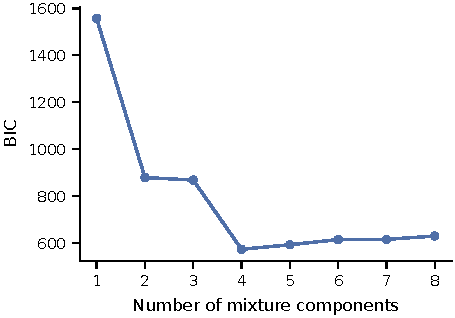
\includegraphics[width=0.5\textwidth]{../figures/figA2_gmm_bic.pdf}
\caption{Bayesian information criterion of Gaussian mixture models fitted to standardised log consumption-based \COtwo{} per person and mean social attainment (country-period means). Lower values indicate a better trade-off between fit and complexity.}
\label{fig:gmm}
\end{figure}

% ======================================================================
\section{Reproducibility}\label{app:repro}

The analysis is implemented as a Python package, run with a single command. The pipeline performs the following steps in order:
\begin{enumerate}
\item It deletes all previous outputs, so that every result file comes from the current run.
\item It loads the raw input files, whose SHA-256 checksums are recorded, and builds the country-year panel. This involves selecting the sample by ISO code and population, merging the sources and applying the interpolation rules.
\item It computes the attainment ratios, overshoot and configurations, for each year and for period averages.
\item It runs all analyses with fixed random seeds: configurations and transitions, the carbon requirement, fixed-effects and long-difference models, decoupling and scenarios, the mixture check and the robustness specifications.
\item It writes every result as a CSV file, every table as a \LaTeX{} file, every figure as PDF and PNG, and every number quoted in the text as a \LaTeX{} macro, which the manuscript reads.
\end{enumerate}

The test suite checks:
\begin{itemize}
\item that the sample contains only UN member states and Palestine, includes known members and meets the population rule;
\item that the panel is a complete, duplicate-free country-year grid and that the periods neither overlap nor mislabel their years;
\item that GDP is in constant purchasing-power-parity terms;
\item that interpolation never extrapolates and respects its gap limits;
\item that each attainment ratio points in the right direction and that zero mortality counts as full attainment;
\item that the classification rules behave correctly, including with missing data and at the tolerance cut-off;
\item that the carbon requirement estimators recover known values from simulated data;
\item that failed logistic fits are detected;
\item that the decoupling classification and scenario arithmetic are correct;
\item that the generated numbers file is valid.
\end{itemize}
Three further checks are part of the package. A static check of the manuscript confirms that every number macro used in the text is defined and every defined macro is used, that every citation exists in the bibliography and every bibliography entry is cited, and that every number typed directly in the text (rather than read from a macro) has been reviewed and assigned to a category such as threshold, definition, label, notation or quoted literature value. An independent re-implementation, written without the analysis package and using only the raw files, re-derives the sample sizes, configuration shares, transitions, foundation crossers, frontier, carbon requirement and its trend, robustness levels, decoupling counts, scenarios and fixed-effects coefficients, and compares each with the numbers in the text; all 54 comparisons agree. Finally, the social indicators in the World Development Indicators extract were compared with the October 2026 release from the World Bank's data service for the 18 countries whose classification is closest to a threshold (410 country-year values). Life expectancy and unemployment were identical, electricity access differed in one value by 0.1 percentage points, and under-5 mortality had been revised by up to 2 deaths per 1{,}000 live births in the newer release. Replacing the extract's values by the newer ones changes no classification.

The complete pipeline was run from scratch in three environments: the development environment (Python 3.13); a fresh virtual environment built only from the pinned package versions (Python 3.13); and a fresh environment on Python 3.11 with the newest compatible library versions. In each run the input checksums were verified, all tests passed, the manuscript check passed and the independent re-implementation agreed on all comparisons. The two runs with the pinned versions produced byte-identical numbers, tables, result files and analysis panel. The Python 3.11 run produced identical numbers and tables; five of its result files differ from the others only in the last digits of floating-point values (by less than $10^{-9}$), which do not affect any reported number. Rendered figure images can differ by a few pixels between environments because of font rasterisation; the data they plot are identical.
